% \documentclass{article}

% \usepackage{algorithm}
% \usepackage{algpseudocode}
% \usepackage{amsmath, amssymb, amsthm}
% \usepackage[letterpaper, margin=1in]{geometry}
% \usepackage{authblk}
% \usepackage{float}
% \usepackage{caption}
% \usepackage{subcaption}
% \usepackage{graphicx}
% \usepackage{hyperref}
% \usepackage{enumerate}

\documentclass[11pt]{amsart}
% Standard letter size paper with 1inch margins
\usepackage[letterpaper, margin=1in]{geometry}
\usepackage{algorithm, algpseudocode}
\usepackage{float}
\usepackage{caption}
\usepackage{amsmath, amssymb, amsthm, amsaddr}
\usepackage{enumerate, subcaption, graphicx, hyperref}
\usepackage{subcaption}

\title{AMATH 482: Homework 4}
\author{Rohan Pandey} % first and last name
\address{University of Washington, Seattle, WA
\\ \texttt{rpande@uw.edu}}
\date{\today} % you can also just type the date instead of "\today"
\begin{document}

\begin{abstract}
This assignment explores Fully Connected Neural Networks (FCNs) and Deep Neural Networks (DNNs) for image classification using the FashionMNIST dataset. The dataset has 60,000 training images and 10,000 test images, each of size 28x28 pixels.

We performed hyperparameter tuning, comparing different optimizers (SGD, Adam, RMSProp), weight initialization methods (Xavier Normal, Kaiming (He) Uniform, Random Normal), and regularization techniques such as Dropout and Batch Normalization. Our experiments analyzed model convergence, overfitting, and generalization.

The final results include training loss curves, accuracy trends, and insights into the most effective configurations for FashionMNIST classification.
\end{abstract}

\maketitle 

\section{Introduction and Overview}\label{sec:Introduction}
Image classification is one of the fundamental tasks in computer vision and has experienced significant advancements with the advent of deep learning. Deep neural networks, by learning hierarchical representations of data, have outperformed traditional methods in various applications. In this assignment, we explore the use of Fully Connected Neural Networks (FCNs) for classifying images from the FashionMNIST dataset, a modern and more challenging alternative to the classic MNIST dataset \cite{xiao2017fashion}. 


\section{Theoretical Background}\label{sec:theory}
% Include theoretical details, such as network architectures, loss functions, and optimization techniques.
Fully Connected Neural Networks (FCNs) consist of layers that perform linear transformations followed by non-linear activations to learn hierarchical representations of data. In each layer, the network computes a weighted sum of its inputs, adds a bias, and then applies a non-linear function (commonly the Rectified Linear Unit, ReLU) to capture complex features. The ReLU activation function is also defined below. For classification tasks, the final layer outputs a vector of raw scores (logits), which are then converted into a probability distribution using the softmax function:
\begin{align}
\text{ReLU}(x) = \max(0, x)\\
\sigma(\mathbf{z})_i = \frac{e^{z_i}}{\sum_{j=1}^{C} e^{z_j}},
\end{align}
where $C$ denotes the number of classes \cite{Goodfellow-et-al-2016}. This transformation allows the network to produce interpretable probabilities for each class.

The performance of the network is evaluated using the Cross-Entropy Loss, which measures the dissimilarity between the predicted probability distribution and the true one-hot encoded labels:
\[
\mathcal{L} = -\sum_{i=1}^{C} y_i \log\big(\sigma(\mathbf{z})_i\big),
\]
ensuring that lower loss values correspond to predictions that are closer to the true labels \cite{Goodfellow-et-al-2016}.

To improve generalization and mitigate overfitting, regularization techniques such as \textbf{dropout} are employed. Dropout randomly deactivates a fraction of neurons during training, which forces the network to learn redundant representations and reduces reliance on any single neuron \cite{srivastava2014dropout}. Additionally, proper weight initialization is crucial for stable training. Methods like Xavier (Glorot) initialization and Kaiming (He) initialization are designed to maintain consistent variance of activations across layers, thereby helping to prevent the vanishing or exploding gradient problem \cite{he2015delving}.

Together, these concepts—layer transformations with non-linear activations, probability mapping via softmax, error quantification using cross-entropy loss, dropout regularization, and robust weight initialization—form the foundation for training effective FCNs for image classification tasks.





\section{Algorithm Implementation and Development}\label{sec:algorithms}
Below is the high-level algorithm implementation for the tasks performed in this assignment.
\begin{algorithm}[H]
    \caption{FCN Training and Hyperparameter Tuning for FashionMNIST}
    \begin{algorithmic}[1]
        \State \textbf{Input:} FashionMNIST dataset, hyperparameters: \texttt{learning\_rate}, \texttt{epochs}, \texttt{batch\_size}, \texttt{hidden\_layers}
        \State \textbf{Output:} Trained model and performance metrics
        
        \State \textbf{/* Data Loading and Preprocessing */}
        \State Load FashionMNIST dataset, normalize, split into Training, Validation, and Test sets.
        \State Reshape images to 784-dimensional vectors.
        
        \State \textbf{/* Task 2: Baseline Model Training */}
        \State Initialize FCN model with hidden layers (e.g., $[128, 64]$), Cross-Entropy loss, and SGD optimizer.
        \For{epoch = 1 to \texttt{epochs}}
            \State Train model on batches, update weights via backpropagation.
            \State Compute training loss and validation accuracy.
        \EndFor
        \State Evaluate final model on Test set.
    
        \State \textbf{/* Task 3: Hyperparameter Tuning */}
        \For{optimizer $\in$ \{SGD, RMSProp, Adam\}, dropout\_rate $\in$ \{0.0, 0.5\}, init\_method $\in$ \{Random, Xavier, Kaiming\}}
            \State Initialize FCN with corresponding settings, train, and evaluate.
        \EndFor
        \State Train FCN with Batch Normalization.
    
        \State \textbf{/* Results and Reporting */}
        \State Plot loss and accuracy curves, summarize test accuracies across experiments.
    \end{algorithmic}
\end{algorithm}    

\section{Computational Results}\label{sec:results}
% Include your plots, tables, and discussion of results here.

First we can talk about the baseline model. This was after finding a working configuration of the FCN model that has an adjustable number of hidden layers and neurons in each layer with relu activation. Recall that FCN stands for Fully Connected Networks. The loss curve as well as its validation accuracy is shown below in Figure \ref{fig:baseline}.

\begin{figure}[H]
    \centering
    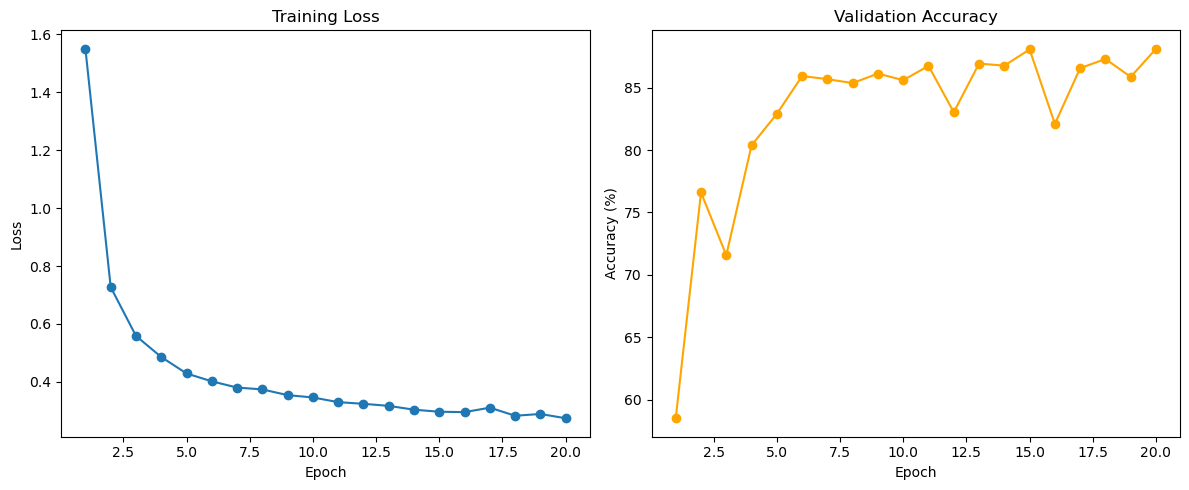
\includegraphics[width=0.75\textwidth]{baseline.png}
    \caption{FCN Baseline Model: Loss and Validation Accuracy with Test Accuracy of $ 87.03\%$}
    \label{fig:baseline}
\end{figure}

The way I was able to achieve this accuracy was by increasing epochs as well as learning rate, although I strongly believe that epochs was more harmful than helpful as we can see around epoch 12 and 15 the accuracy dropped suddenly. This is a sign of overfitting.

\subsection{Hyperparameter Tuning}

\subsubsection{Optimizers}

We then worked on tuning our parameters on the baseline model, using RMSProp, Adam and SGF optimizers. The results of this tuning are shown below, we have the plots of loss curves, and also a table detailing the test accuracies. Note the legend on the plots to see which optimizer is which.

\begin{figure}[H]
    \centering
    \begin{subfigure}{0.55\textwidth}
        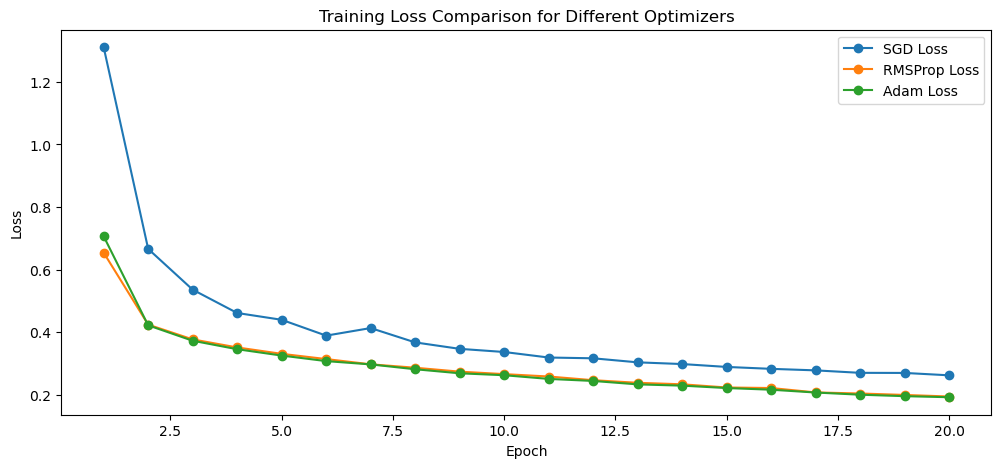
\includegraphics[width=\textwidth]{optimizer_loss.png}
        \caption{Loss Curves}
    \end{subfigure}
    \begin{subfigure}{0.55\textwidth}
        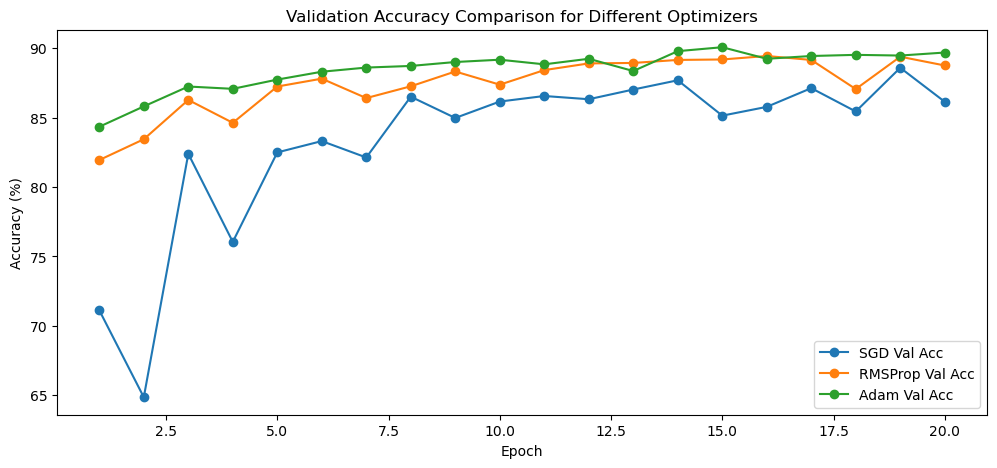
\includegraphics[width=\textwidth]{optimizer_accuracy.png}
        \caption{Validation Accuracy}
    \end{subfigure}
    \caption{FCN Optimizer Tuning: Loss and Validation Accuracy}
    \label{fig:optimizer}
\end{figure}

\begin{table}[H]
    \centering
    \begin{tabular}{|c|c|}
    \hline
    \textbf{Optimizer} & \textbf{Test Accuracy (\%)} \\ \hline
    SGD & 85.26 \\ \hline
    RMSProp & 87.34 \\ \hline
    Adam & 88.52 \\ \hline
    \end{tabular}
    \caption{Test Accuracies for Different Optimizers}
    \label{tab:optimizer}
\end{table}

From \ref{tab:optimizer}, we can see that Adam is the best optimizer for this model, with a test accuracy of $88.52\%$. This is followed by RMSProp and then SGD. I think this might be because Adam is a combination of RMSProp and Momentum, which allows it to converge faster and more efficiently.

\subsubsection{Regularization}

We then used Dropout regularization to prevent overfitting. The results of this tuning are shown below, we have the plots of loss curves, and also a table detailing the test accuracies. Note the legend on the plots to see which dropout rates we used and what the results were.

\begin{figure}[H]
    \centering
    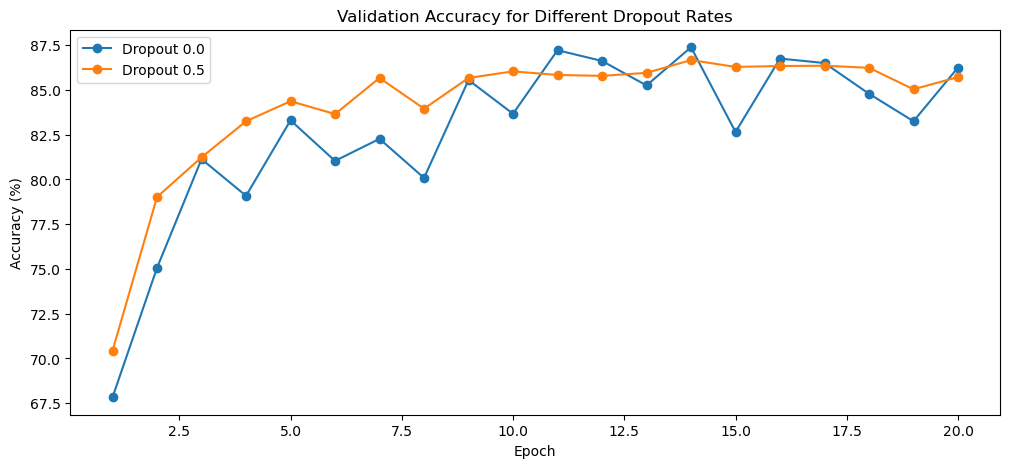
\includegraphics[width=0.75\textwidth]{regularization.png}
    \caption{FCN Dropout Regularization: Loss and Validation Accuracy}
    \label{fig:regularization}
\end{figure}

\begin{table}[H]
    \centering
    \begin{tabular}{|c|c|}
    \hline
    \textbf{Dropout Rate} & \textbf{Test Accuracy (\%)} \\ \hline
    0.0 & 85.26 \\ \hline
    0.5 & 84.59 \\ \hline
    \end{tabular}
    \caption{Test Accuracies for Different Dropout Rates}
    \label{tab:regularization}
\end{table}

From \ref{tab:regularization}, we can see that Dropout regularization did not help our model. This is because Dropout is a technique that randomly sets a fraction of input units to zero at each update during training time, which usually helps with overfitting. However, in this case, it seems to have made the model worse.

\subsubsection{Initialization}

We then used different weight initialization methods such as Random Normal, Xavier Normal, and Kaiming (He) Uniform. The results of this tuning are shown below, we have the plots of loss curves, and also a table detailing the test accuracies. Note the legend on the plot as we have plotted all the weight initialization methods on the same plot.

\begin{figure}[H]
    \centering
    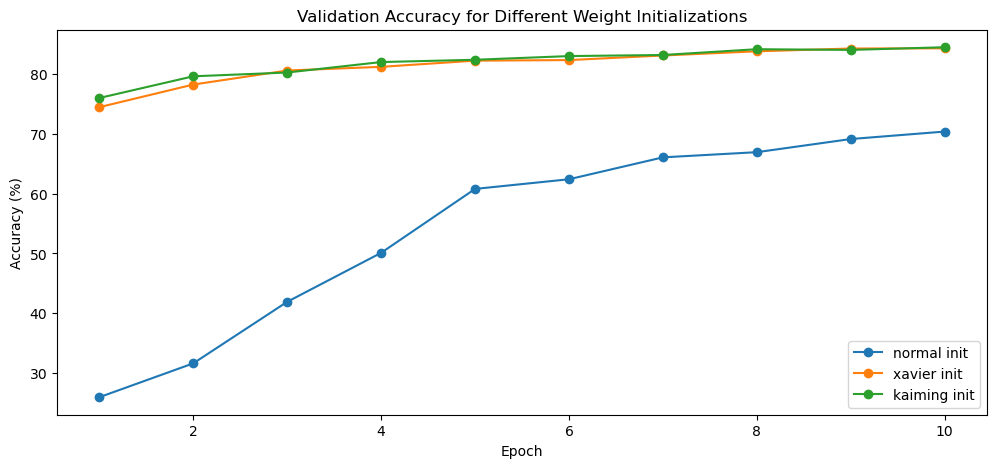
\includegraphics[width=0.5\textwidth]{initialization.png}
    \caption{FCN Weight Initialization: Loss and Validation Accuracy}
    \label{fig:initialization}
\end{figure}

\begin{table}[H]
    \centering
    \begin{tabular}{|c|c|}
    \hline
    \textbf{Initialization Method} & \textbf{Test Accuracy (\%)} \\ \hline
    Random Normal & 69.40 \\ \hline
    Xavier Normal & 83.18 \\ \hline
    Kaiming (He) Uniform & 83.68 \\ \hline
    \end{tabular}
    \caption{Test Accuracies for Different Weight Initialization Methods}
    \label{tab:initialization}
\end{table}

From \ref{tab:initialization}, we can see that Kaiming (He) Uniform initialization is the best weight initialization method for this model, with a test accuracy of $83.68\%$. This is followed by Xavier Normal and then Random Normal. This is because Kaiming (He) Uniform initialization is specifically designed for ReLU activation functions, which we are using in our model. Alternatively, something that I found through testing was that the Kaiming initializer was not learning at all if the learning rate was too high. Originally it was set to $0.1$, and I had to reduce it to $0.01$ to get the model to learn otherwise the test accuracy was stuck at $10\%$ for all $20$ epochs, as an extra precaution I also reduced the number of epochs to $10$ to prevent overfitting.


\subsubsection{Normalization}


Lastly, we included Batch Normalization in our model. In addition to the training loss curve and the validation accuracy achieved by the normalization techniques, I also plotted the Baseline models loss curve and validation accuracy for comparison. The results are shown below.

\begin{figure}[H]
    \centering
    \begin{subfigure}{0.45\textwidth}
        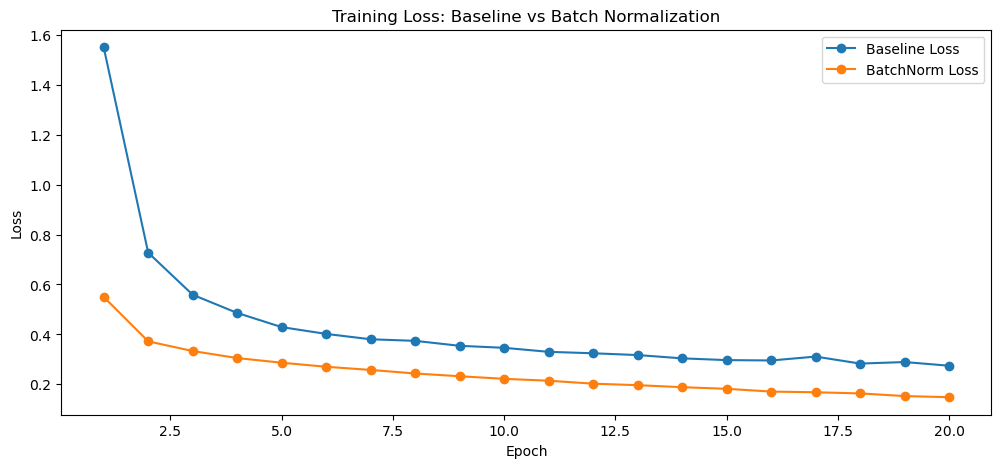
\includegraphics[width=\textwidth]{normalization_loss.png}
        \caption{Loss Curves}
    \end{subfigure}
    \begin{subfigure}{0.45\textwidth}
        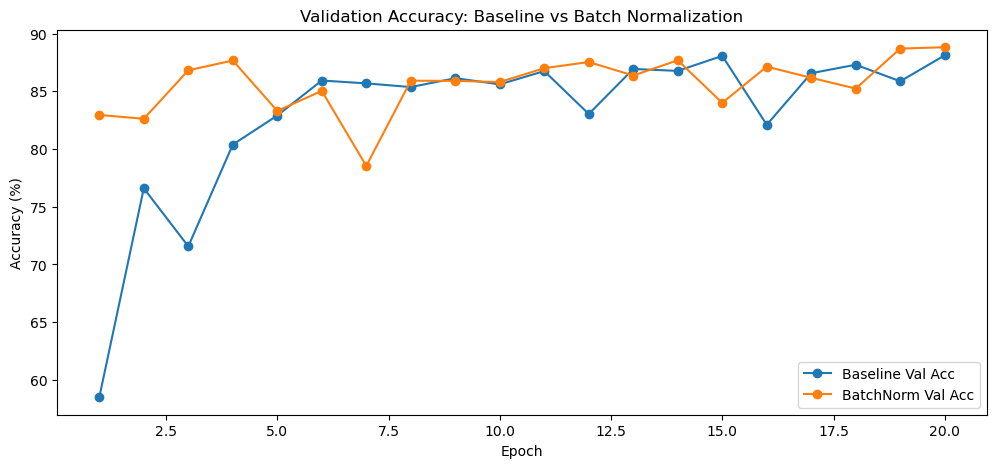
\includegraphics[width=\textwidth]{normalization_accuracy.png}
        \caption{Validation Accuracy}
    \end{subfigure}
    \caption{FCN Normalization Techniques: Loss and Validation Accuracy of $88.01 \%$}
    \label{fig:normalization}
\end{figure}

Clearly we can see that the baseline loss curve is greater than the loss curve of the Batch Normal loss curve. Similarly, the validation accuracy of the baseline model is more scattered in comparison to the Batch Normal which has a bit of variance in the initial epochs but then stabilizes. The test accuracy of the Batch Normal model is $88.01\%$ which is better than the baseline model. This is because Batch Normalization normalizes the output of a previous activation layer by subtracting the batch mean and dividing by the batch standard deviation. This has the effect of stabilizing and accelerating the learning process, and also allows for higher learning rates.



\section{Summary and Conclusions}\label{sec:conclusions}
% Wrap up your report with a brief summary of what you did and what you discovered. 
% Finish with some conclusions and possibly future directions if any.

In this assignment, we explored Fully Connected Neural Networks (FCNs) for image classification using the FashionMNIST dataset. We implemented a baseline model and performed hyperparameter tuning to optimize the model's performance. Our experiments included comparing different optimizers, weight initialization methods, regularization techniques, and normalization methods.

Our results showed that Adam optimizer outperformed SGD and RMSProp, achieving a test accuracy of $88.52\%$. We also found that Kaiming (He) Uniform initialization was the most effective weight initialization method, with a test accuracy of $83.68\%$. Dropout regularization did not improve the model's performance, while Batch Normalization significantly enhanced the model's accuracy to $88.01\%$.

In conclusion, our experiments demonstrated the importance of hyperparameter tuning and the impact of different optimization techniques on model performance. Future work could involve exploring more advanced architectures such as Convolutional Neural Networks (CNNs) for image classification tasks, as well as investigating the effects of other regularization techniques and normalization methods on model performance.

\section*{Acknowledgements}
The author is thankful to Professor Frank for providing the materials and resources needed to complete this assignment. The author is also thankful to the peers Eric Ye and Chenab and Brighton for collaborative work and brainstorm sessions for the Theoretical Background section and visualizations in Python.

\bibliographystyle{abbrv}
\bibliography{HW_References} % Ensure the bibliography file is correctly referenced.

\end{document}
